\section{Neutrino detection}
%TODO: Write down detection process. This section should be written carefully. 
% Specify the guys going into NC and CC. 
% First line only true for CC
% In next lines ,detail the detection process (interaction with detector matter osv). 
% Specify which are occurring in tracks and cascades.
We always observe neutrinos indirectly through their associated charged lepton. 
Regardless of the type of interaction (charged current via the $W$ boson, or neutral current
via the $Z$), a charged lepton exits with altered properties. The lepton is then detected, and the properties of the neutrino involved in the 
interaction are then deduced. This deduction will be imperfect, and this introduces complexities that we will handle in Ch.~\ref{ch:ICmethod}. 

In this work, we only study the detectors handled by the IceCube collaboration. They are of Cherenkov type, which means that they detect 
the secondary charged lepton by its emitted Cherenkov light, produced from its travel through the Antarctic ice. 
To detect the Cherenkov light, 60 Digital Optical Modules (DOMs) are placed on a long string up to \SI{17}{\metre} apart. 86 of these strings are then lowered
into \SI{2.5}{\km} deep boreholes in the ice. The holes are then sealed by refreezing the ice, resulting in a total of 5160 DOMs in a volume of approximately \SI{1}{\km^3}~\cite{weaverThesis}.

The strings and DOMs are not spaced evenly, making some parts of the detector more sensitive to certain energy ranges than others.
8 strings packed more tightly than the other 78, making that part of the detector sensitive to neutrino energies down to single-digit \si{\GeV}. This detector is referred to DeepCore. DeepCore will be treated as a separate and independent detector from the rest, which
retains the name IceCube. A view of the current setup can be seen in Fig.~\ref{fig:array}. In this work, we consider DeepCore data between \SIrange{5.6}{56}{\GeV} and IceCube data in the range \SIrange{0.5}{10}{\TeV}.
\begin{figure}
    \centering
    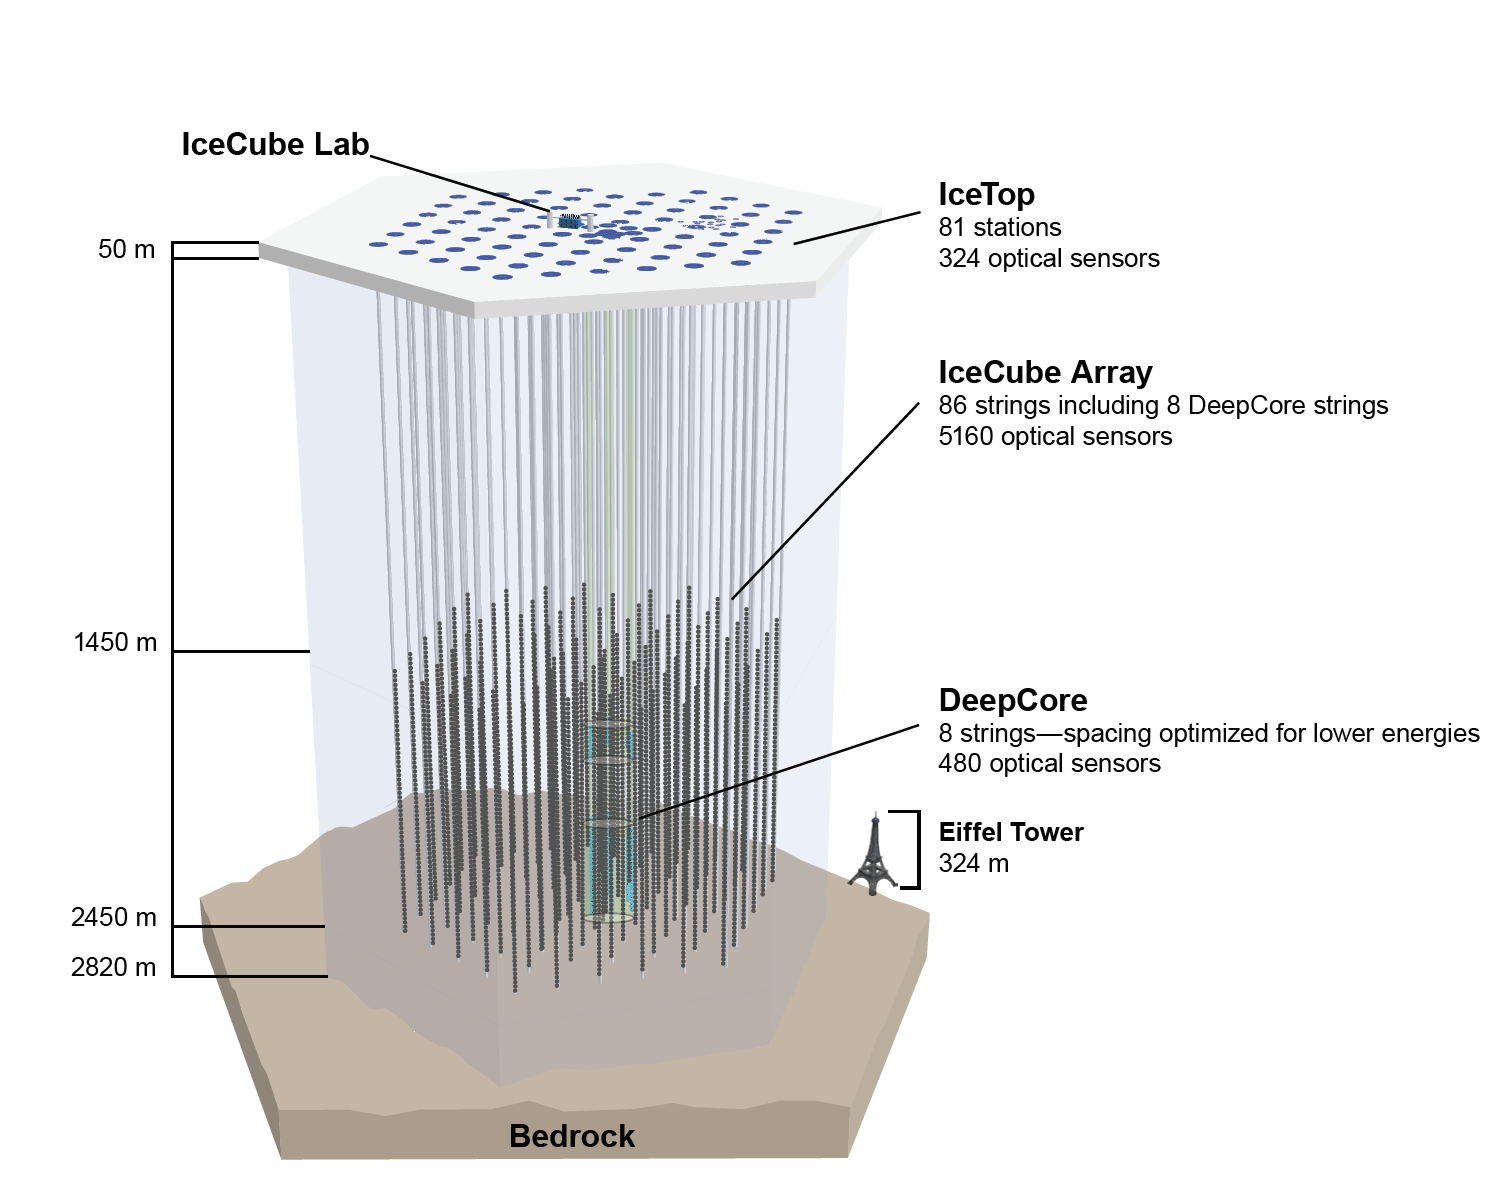
\includegraphics[width=0.8\textwidth]{figures/icecube2.png}
    \caption{View of the full IceCube array, with the Eiffel tower for scale.}\label{fig:array}
\end{figure}

If the charged leptons interact heavily with the ice, they will travel a short distance and emit a localized flash of 
Cherenkov light. This event is referred to as a cascade. The neutral current interactions involve quarks, which recoils and produces
showers of hadrons. Also, charged current $\ne$ interactions also produce cascades. A cascade event 
is shown in Fig.~\ref{fig:events_cascade}.
% S wanted to remove below. Why?
If the charged leptons don't interact as much in the ice, they penetrate a larger part of it, emitting light and tertiary particles
as they go. This event is referred to as a track and is often due to charged current muon interactions. A track event 
is shown in Fig.~\ref{fig:events_track}. 
%TODO: numbers on how often^. Write about which particles appear where

\begin{figure}\label{fig:events}
    \begin{center}
        \begin{subfigure}{0.4\textwidth}
            \centering
            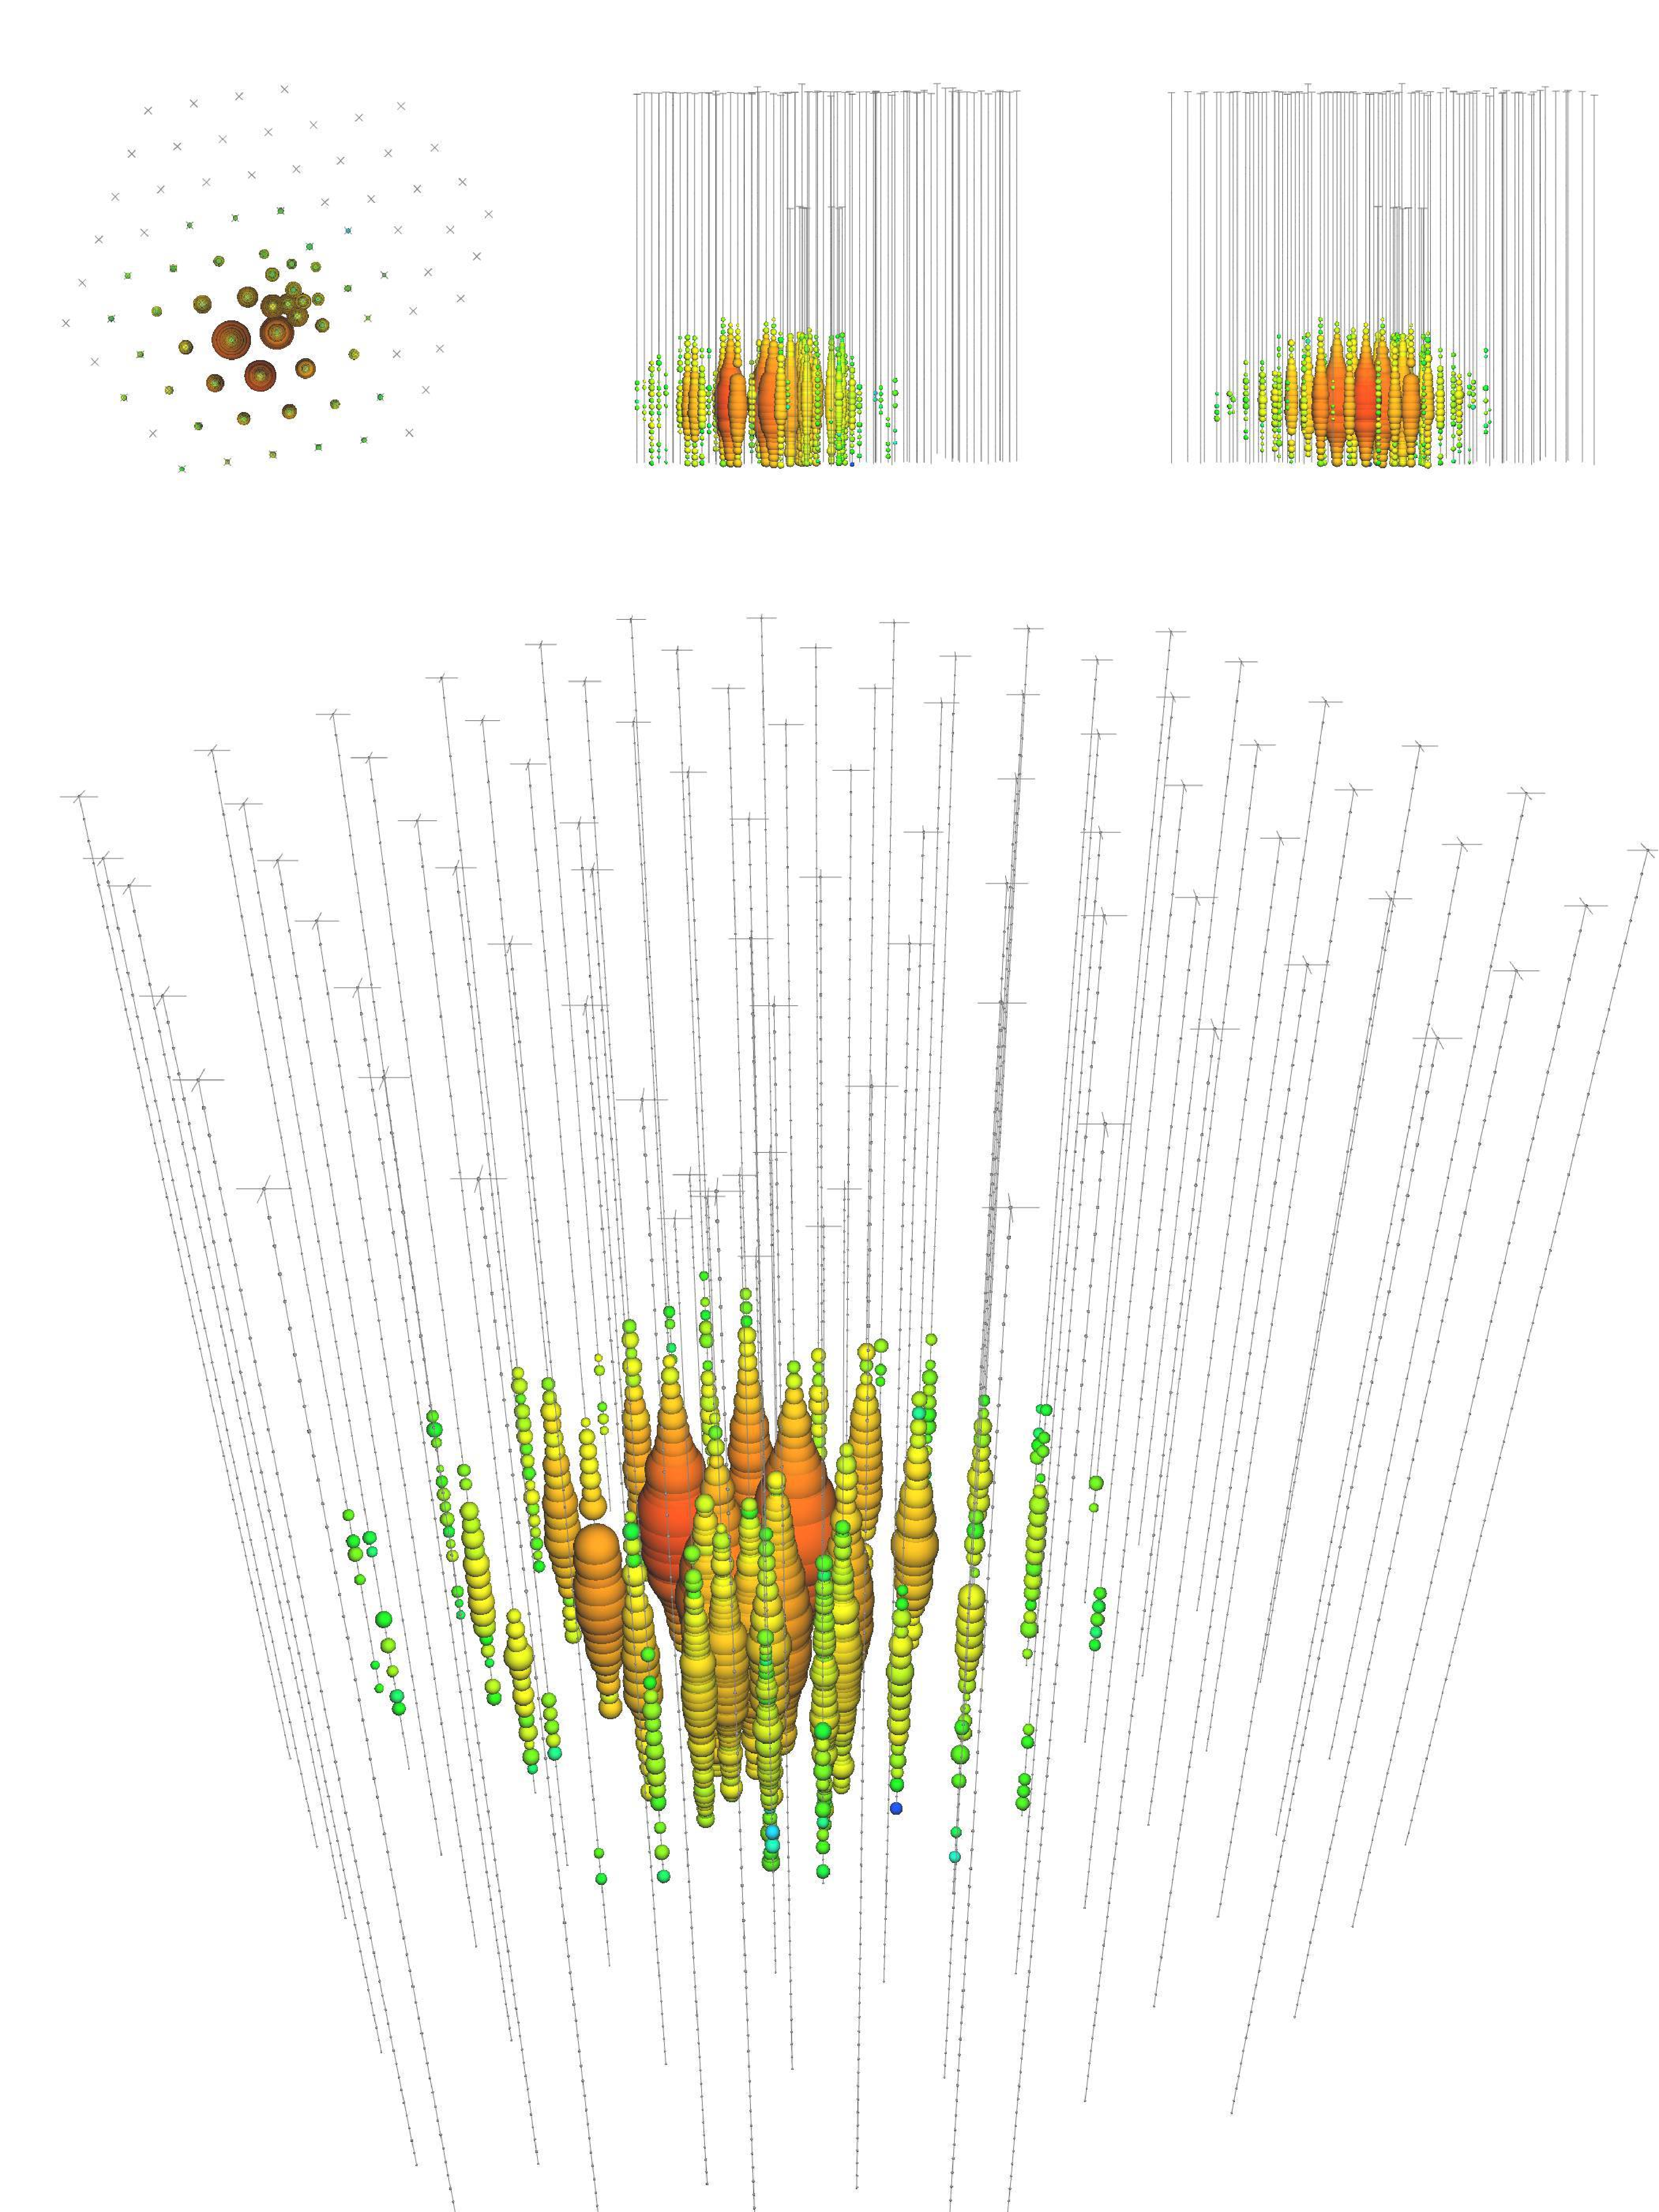
\includegraphics[clip, trim=0cm 0cm 0cm 30cm, width=1\textwidth]{figures/cascade_event.pdf}
            \caption{Event classified as cascade}  
            \label{fig:events_cascade}
          \end{subfigure}
        \begin{subfigure}{0.4\textwidth}
            \centering
            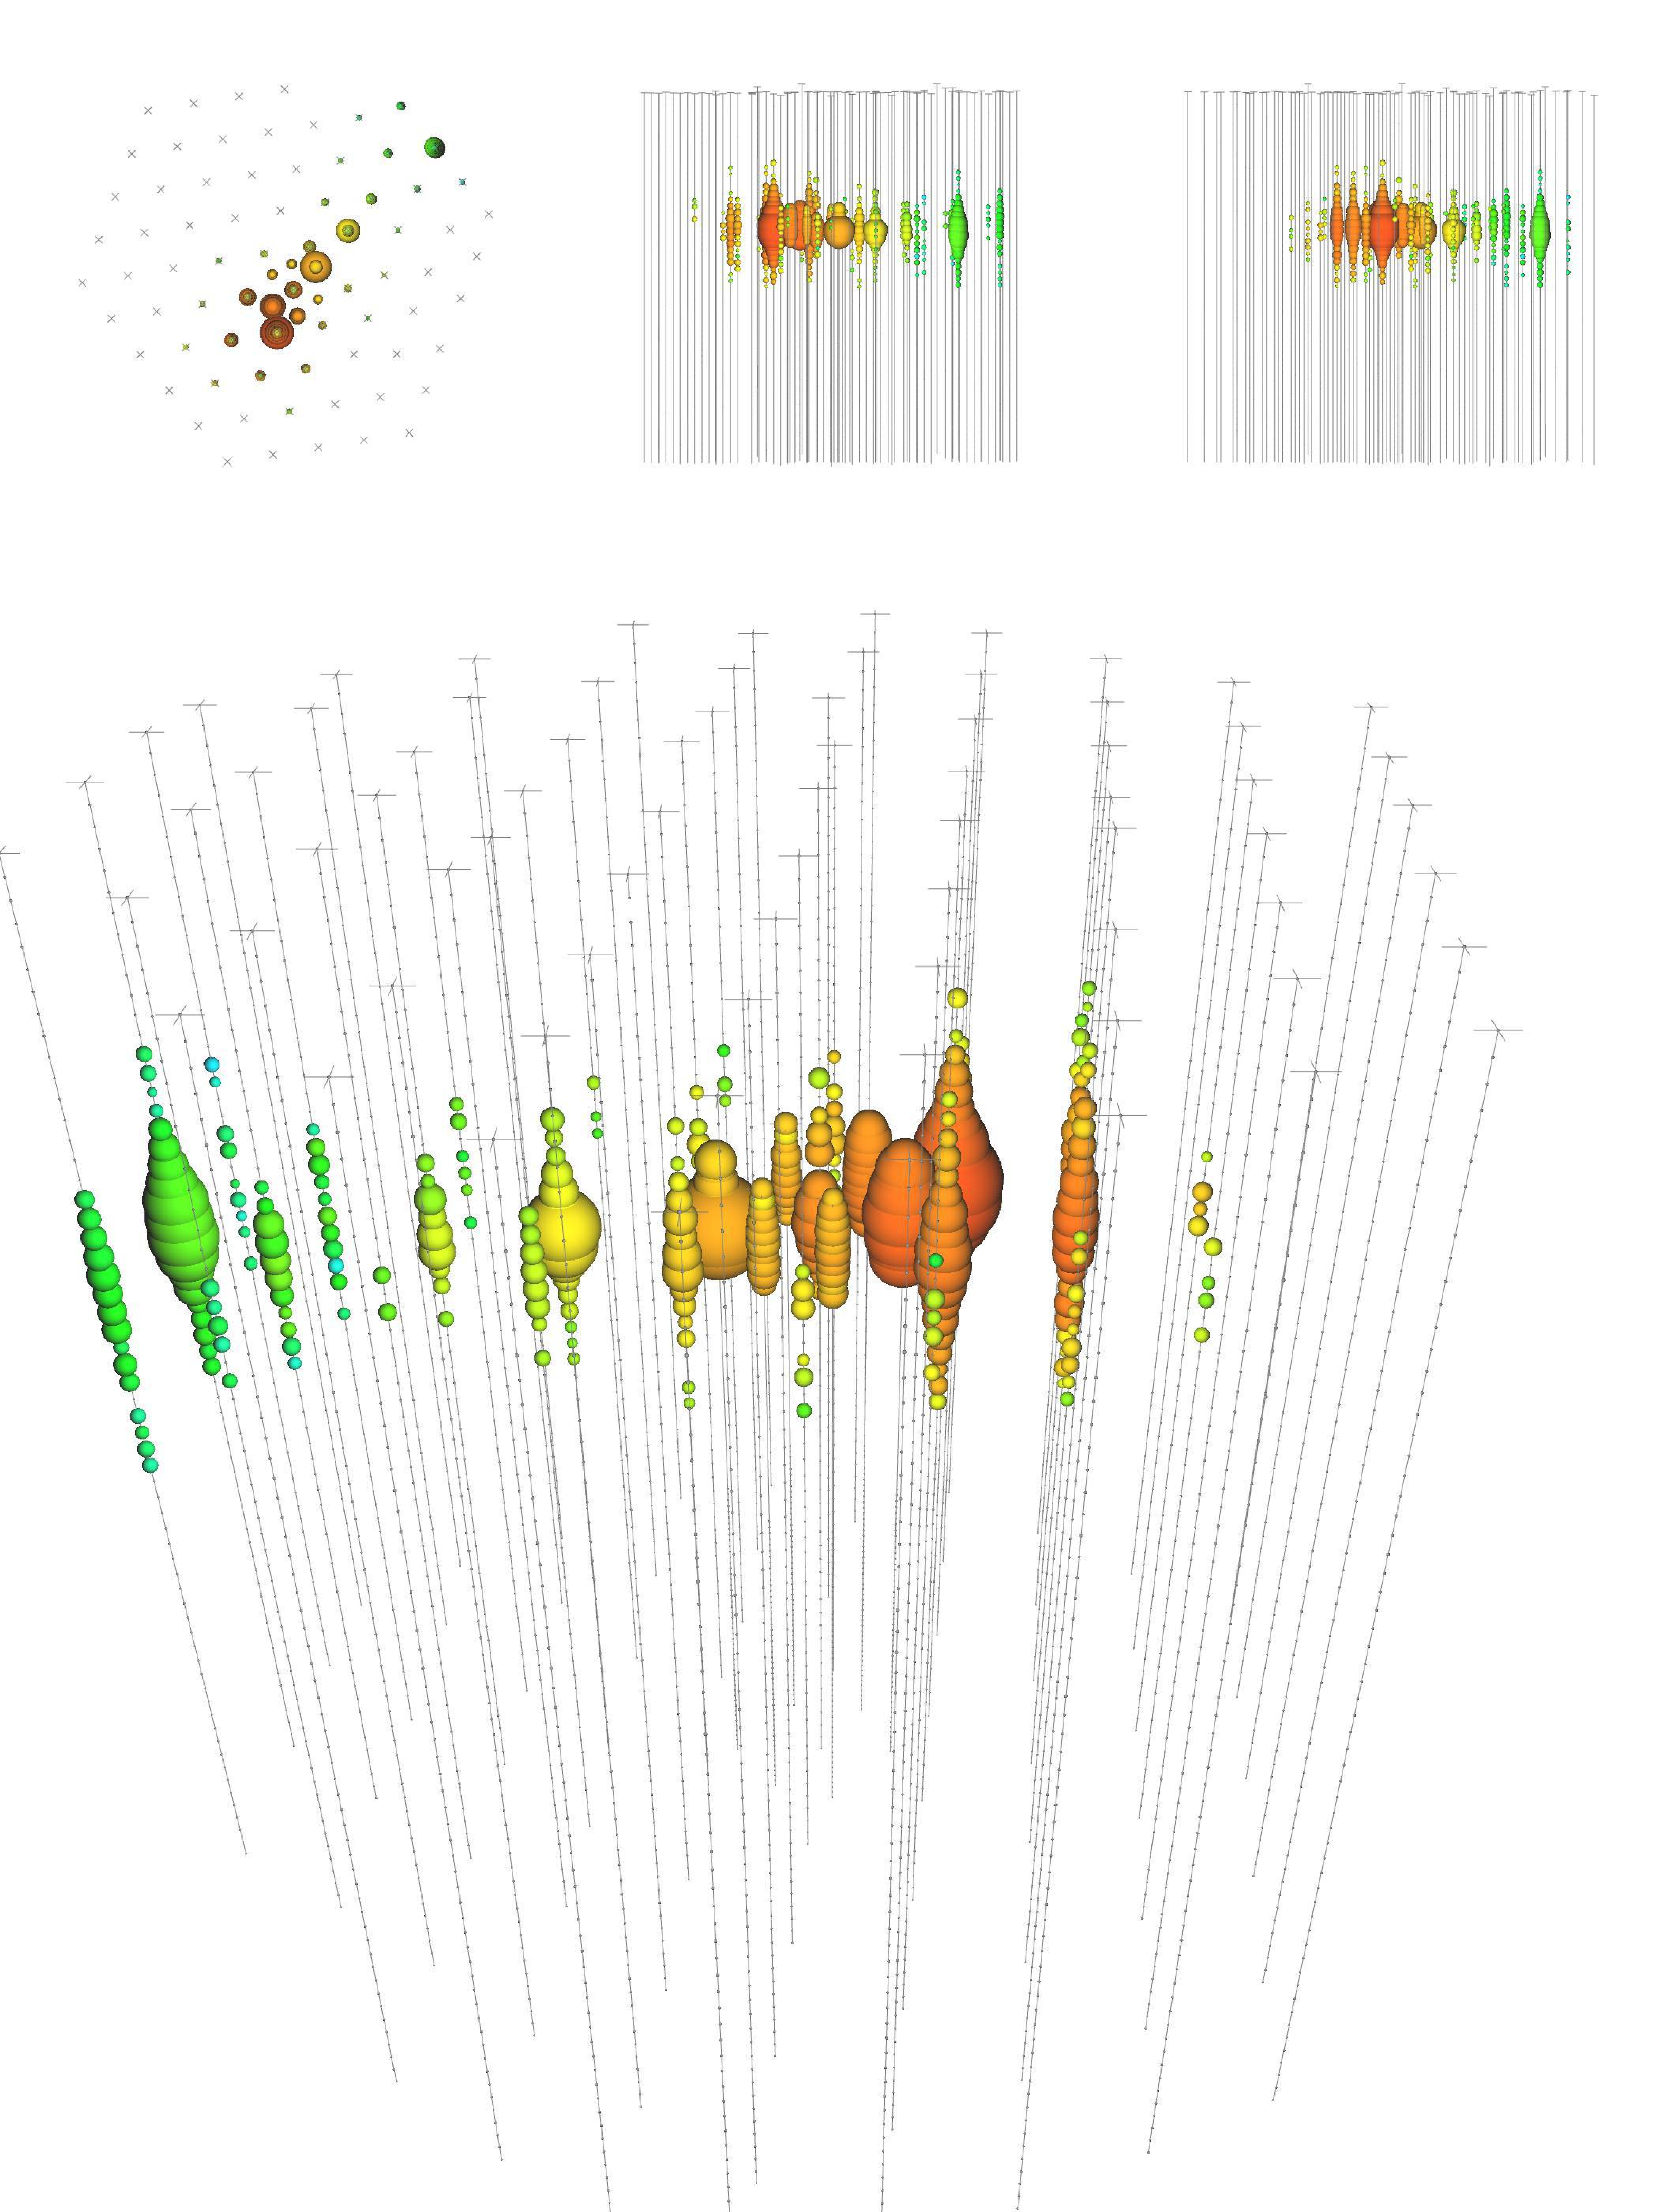
\includegraphics[clip, trim=0cm 0cm 0cm 30cm, width=1\textwidth]{figures/track_event.pdf}
            \caption{Event classified as track} 
            \label{fig:events_track}
        \end{subfigure}
        \caption{The two event types distinguished in the IceCube detector.}
    \end{center}
\end{figure}


In 2017, the PINGU Letter of Intent was published~\cite{PINGUletter}. The `Precision IceCube Next Generation Upgrade' is an upgrade that will 
supplement DeepCore, i.e. boosting the capabilities of neutrino detection at the \si{\GeV} scale. As the PINGU upgrade is not yet financed nor built, we are
not able to use any data from it. However, the collaboration has released preliminary simulations which we will use to see how the upgrade might improve
results from IceCube and DeepCore. The PINGU simulations have the same structure as the DeepCore data, so our analysis referring to DeepCore will
also apply to PINGU except where noted. However, we treat the PINGU detector as independent of the other experiments.

\subsection{Atmospheric Neutrino Flux}
Atmospheric neutrinos originate from cosmic rays composed of high-energy protons interacting with nuclei in the atmosphere.
These interactions ultimately produces pions, which decay as 
\begin{align}\label{eq:pion} %TODO: Incorrect. Add muon decays
    &\pi^+ \to \mu^+ + \nm\,, \quad \pi^- \to \mu^- + \anm \nonumber \\
    &\pi^+ \to e^+ + \ne\,,\,\, \quad \pi^- \to e^- + \ane\,.
\end{align}
In the muonic decay channel, muons are emitted which will be detected by the IceCube detector.

The flux is provided in \cite{hondaData,hondaArticle}, and a selection is shown in Table~\ref{table:flux}.
The flux data is binned in $\cos(\theta_z)$. The fluxes are averaged over the azimuthal direction and solar minimum/maximum. 
The units of the fluxes are given as \si{\per\GeV \per\metre\squared \per\second \per\steradian} and are omitted
from the table for clarity. 
We note that the fluxes for $\nt$ and $\bar{\nu}_{\tau}$ are missing. Kaons do not decay into $\nt$. Thus, we never have to use probabilities in the form 
$P_{\tau \beta}$, since we have no starting atmospheric $\nu_\tau$ flux. 
Interpolating the data yields makes us capable of approximating all four necessary fluxes for a given true energy and true zenith.
The result of $\phi_\mu$ is shown in Fig.~\ref{fig:flux}. We see that the flux is almost entirely zenith independent. This is due to the 
very small cross-section of the neutrinos. For particles interacting through the electromagnetic interaction, we would expect to see a 
large difference between the flux of particles traversing through the whole diameter of the Earth, compared to particles that only penetrate a 
small rim of the crust. Here, however, the flux at the South Pole is almost the same! This does not mean that the oscillation probability will be 
equal. First, the difference in the density profiles introduces wildly different matter effects. 
Secondly, the zenith angle determines the baseline. Completely down-going neutrinos, with $\cos(\theta_z) = 0$ will be produced at an average distance of \SI{15}{\km}
overhead, travel down to the icy sheet of Antarctica, and then penetrate the ice down \SI{2}{\km} to the DOMs~\cite{hondapaper}. 
The energy dependence of the flux is approximately $E^{-2.7}$, so our expected event count at higher energies will suffer from this strong decline in flux.

\begin{table}[h]
    \begin{center}
        \begin{tabular}{lcccccc}
            \hline \hline
            $E$ [\si{\GeV}] &$\phi_\mu$ &$\phi_{\bar{\mu}}$ &$\phi_e$ &$\phi_{\bar{e}}$ & $\cos(\theta_z)$\\
            \hline
            27825 &  \SI{6.06e-12}{} &  \SI{3.17e-12}{} &  \SI{1.56e-13}{} &  \SI{1.04e-13}{} &   [-0.2, -0.1] \\
            247707 &  \SI{5.94e-16}{} &  \SI{2.92e-16}{} &  \SI{1.36e-17}{} &  \SI{8.12e-18}{} &   [-0.7, -0.6] \\
                22 &  \SI{3.33e-02}{} &  \SI{2.78e-02}{} &  \SI{9.57e-03}{} & \SI{7.15e-03}{} &   [-0.3, -0.2] \\
            432876 &  \SI{5.19e-17}{} &  \SI{2.32e-17}{} &  \SI{1.46e-18}{} & \SI{9.83e-19}{} &   [-1.1, -1.0] \\
            64280 &  \SI{1.58e-13}{} &  \SI{8.10e-14}{} &  \SI{3.49e-15}{} &  \SI{2.21e-15}{} &   [-0.4, -0.3] \\
            \hline \hline
        \end{tabular}
    \end{center}
    \caption{A selection of processed atmospheric South Pole fluxes from~\cite{hondaData} by Honda et al.~\cite{hondaArticle}.}\label{table:flux}
\end{table}


\begin{figure}[t]
    \centering
    %TODO: rework
    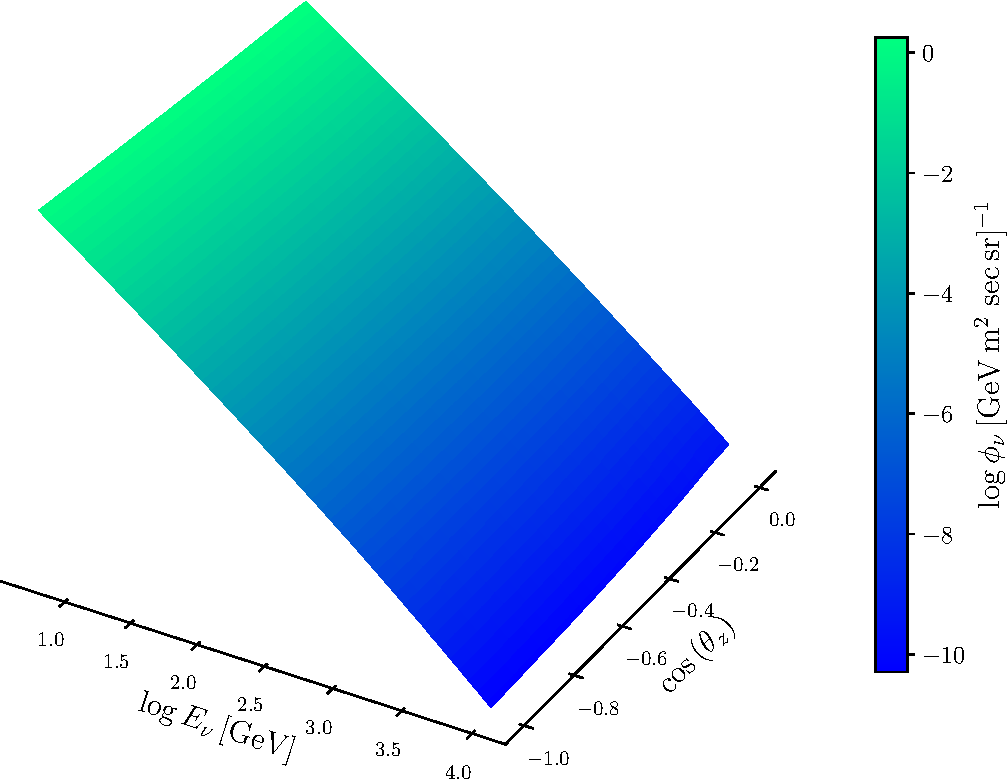
\includegraphics[width=0.9\textwidth]{figures/flux.pdf}
    \caption{Interpolated South Pole atmospheric $\nu_\mu$ flux with data from~\cite{hondaArticle}, displaying a weak 
    zenith angle dependance, but a strong energy dependence. The energy dependence can be parametrized to be approximated by $E^{-2.7}$.}\label{fig:flux}
\end{figure}

We propagate the atmospheric neutrino flux $\phi_\alpha^\text{atm}(E,\theta_z)$ through the Earth.
The oscillation probability $P_{\alpha \beta}$ acts as a weight to the atmospheric flux, yielding the propagated flux for flavor $\beta$ at detector level as 
\begin{align}\label{eq:propFlux}
    \phi_\beta^\text{det} = \sum_\alpha P_{\alpha\beta} \phi_\alpha^\text{atm} \,,
\end{align}
where we sum over the initial lepton flavors $\alpha \in \{e,\mu, \bar{e}, \bar{\mu}\}$.

\subsection{True and Recontstructed Parameters}
After an event has occurred, the IceCube collaboration \emph{reconstruct} the event. 
This means that, given the parameters recorded by the detector, what are their `true' values?
We are interested in two variables: energy and direction. Each event is tagged with a probable energy and zenith angle, 
called the reconstructed parameters $\Ereco$ and $\zreco$, which are the parameters according to the DOMs.
In other words, the collaboration uses the recorded data to backtrack the event, using the reconstructed parameters to approximate the true parameters. 
So a charged lepton hits the DOMs, and we ultimately end up with the associated neutrino's true energy and zenith angle, $\Etrue$ and $\ztrue$. 
The reconstructed parameters are what we are using to analyze the data (because this is what the detector sees), while the true parameters are used in the 
determination of that neutrino's `actual' flux and cross-section (because this is what Nature sees).

How do we then translate between the reconstructed and true parameters? 
In this work, we are using two different methods, which are based on the form of data available to us. 
They will be outlined in Sec.~\ref{ch:ICmethod} and Sec.~\ref{ch:DCmethod}.



% \bibliographystyle{nature}
% \bibliography{ref.bib}
% \end{document}